% Define the top matter
\renewcommand{\moduleTitle}{Data Quality}
\renewcommand{\moduleAuthors}{%
  Sonika Tyagi \mailto{sonika.tyagi@agrf.org.au}
} \renewcommand{\moduleContributions}{%
  Nathan S. Watson-Haigh \mailto{nathan.watson-haigh@awri.com.au}%
}

%  Start: Module Title Page
\chapter{\moduleTitle}
\newpage
% End: Module Title Page

\section{Key Learning Outcomes}

After completing this practical the trainee should be able to:
\begin{itemize}
  \item Assess the overall quality of NGS sequence reads
  \item Visualise the quality, and other associated matrices, of reads to decide
        on filters and cutoffs for cleaning up data ready for downstream analysis
  \item Clean up and pre-process the sequences data for further analysis
\end{itemize}

\section{Resources You'll be Using}
 
\subsection{Tools Used}
\begin{description}[style=multiline,labelindent=0cm,align=left,leftmargin=0.5cm]
  \item[FastQC]\hfill\\
  	\url{http://www.bioinformatics.babraham.ac.uk/projects/fastqc/}
  \item[FASTX-Toolkit]\hfill\\
  	\url{http://hannonlab.cshl.edu/fastx_toolkit/}
  \item[Picard]\hfill\\
  	\url{http://picard.sourceforge.net/}
\end{description}

\section{Useful Links}
 
\begin{description}[style=multiline,labelindent=0cm,align=left,leftmargin=0.5cm]
  \item[FASTQ Encoding]\hfill\\
    \url{http://en.wikipedia.org/wiki/FASTQ_format#Encoding}
\end{description}

% \subsection{Sources of Data}
% TODO Provide a publically available data set used for this module
% \url{http://www.ebi.ac.uk/ena/data/view/ERR022484}\\
% \url{http://www.ebi.ac.uk/ena/data/view/ERR022485}

\newpage

\section{Introduction}

\begin{note}
Going on a blind date with your read set? For a better understanding of the
consequences please check the data quality!
\end{note}

For the purpose of this tutorial we are focusing only on Illumina sequencing
which uses 'sequence by synthesis' technology in a highly parallel fashion.
Although Illumina high throughput  sequencing provides highly accurate sequence
data, several sequence artifacts, including base calling errors and small
insertions/deletions, poor quality reads and primer/adapter contamination are
quite common in the high throughput sequencing data. The primary errors are
substitution errors. The error rates can vary from 0.5-2.0\% with errors mainly
rising in frequency at the 3' ends of reads.

One way to investigate sequence data quality is to visualize the quality scores
and other metrics in a compact manner to get an idea about the quality of a read
data set. Read data sets can be improved by post processing in different ways
like trimming off low quality bases, cleaning up any sequencing adapters and
removing PCR duplicates. We can also look at other statistics such
as, sequence length distribution, base composition, sequence complexity,
presence of ambiguous bases etc. to assess the overall quality of the data set.

Highly redundant coverage ($>$15X) of the genome can be used to correct sequencing
errors in the reads before assembly and errors. Various k-mer based error
correction methods exist but are beyond the scope of this tutorial.

\section{Prepare the Environment}

\begin{information}
To investigate sequence data quality we will demonstrate tools called FastQC
and FASTX-Toolkit. FastQC will process and present the reports in a visual manner.
Based on the results, the sequence data can be processed using the FASTX-Toolkit.
We will use one data set in this practical, which can be found in the QC
directory on your desktop.
\end{information}

\begin{steps}
Open the Terminal and go to the directory where the data are stored:
\begin{lstlisting}
cd ~/QC/
pwd
\end{lstlisting}

At any time, help can be displayed for FastQC using the following command:
\begin{lstlisting}
fastqc -h
\end{lstlisting}

\end{steps}


\section{Quality Visualisation}

\begin{information}
We have a file for a good quality and bad quality statistics. FastQC generates
results in the form of a zipped and unzipped directory for each input file.
\end{information}

\begin{steps}
Execute the following command on the two files:
\begin{lstlisting}
fastqc -f fastq bad_example.fastq 
fastqc -f fastq good_example.fastq
\end{lstlisting}

View the FastQC report file of the dab data using a web browser such as
firefox.

\begin{lstlisting}
firefox bad_example_fastqc/fastqc_report.html &
\end{lstlisting}

\end{steps}

\begin{note}
The report file will have a Basic Statistics table and various graphs and tables
for different quality statistics. E.g.:
\end{note}

\begin{table}[H]
  \centering
  \caption{FastQC Basic Statistics table}
    \begin{tabular}{ll}
    \toprule
    Filename & bad\_example.fastq \\
    \midrule
    File type & Conventional base calls \\
    Encoding & Sanger / Illumina 1.9 \\
    Total Sequences & 40000 \\
    Filtered Sequences & 0 \\
    Sequence length & 100 \\
    \%GC  & 48 \\
    \bottomrule
    \end{tabular}
  \label{tab:badexampleuntrimmed}
\end{table}

\begin{figure}[H]
\centering
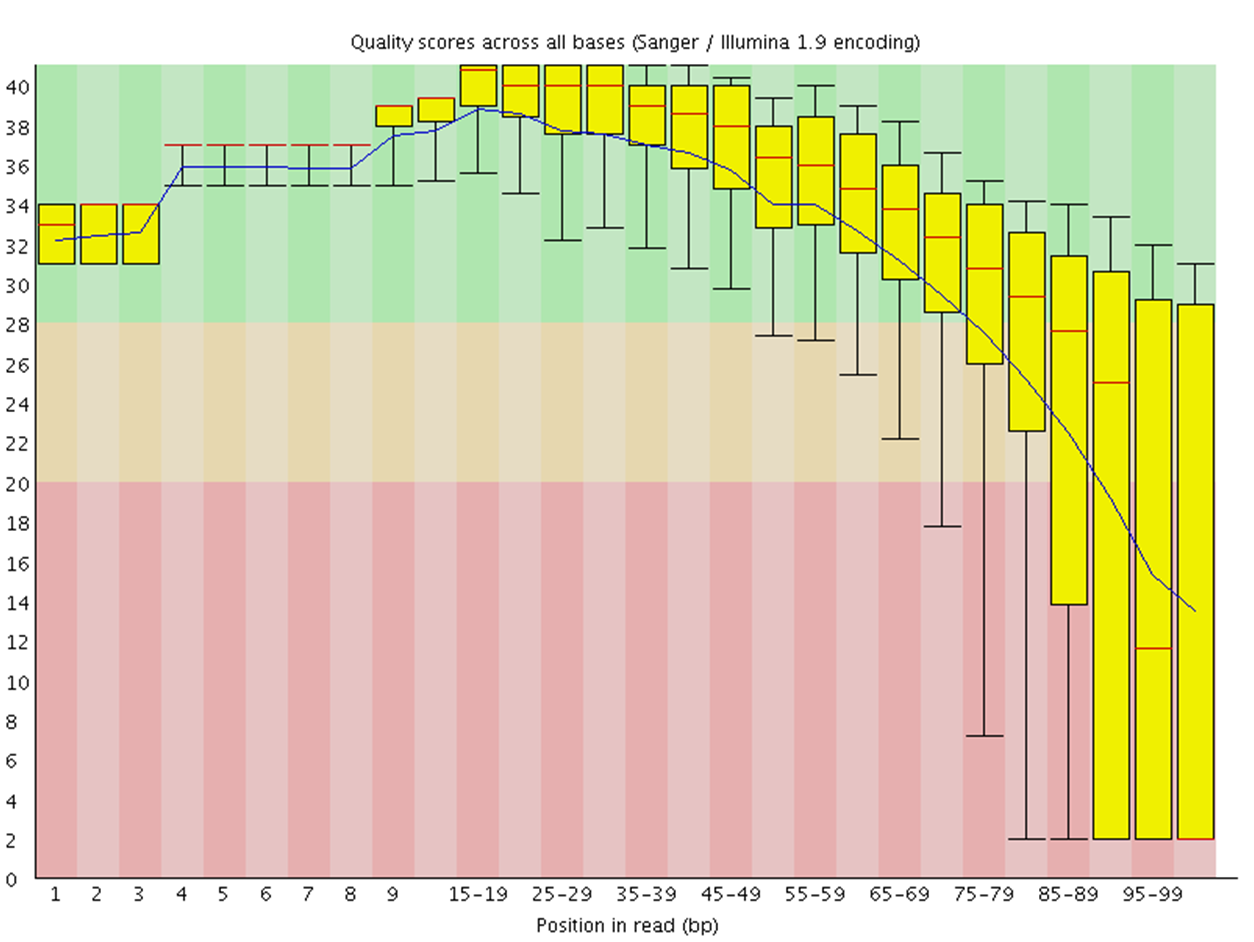
\includegraphics[width=0.8\textwidth]{ngs-qc/bad_example.png}
\caption{Per base sequence quality plot for \texttt{bad\_example.fastq}.}
\label{fig:bad_example_untrimmed_plot}
\end{figure}

\begin{information}
A Phred quality score (or Q-score) expresses an error probability.  In particular, it
serves as a convenient and compact way to communicate very small error
probabilities.
The probability that base $A$ is wrong ($P(\sim A)$) is expressed
by a quality score, $Q(A)$, according to the relationship:
\\\\
$Q(A) =-10 log10(P(\sim A))$
\\\\
The relationship between the quality score and error probability is demonstrated
with the following table:

\begin{table}[H]
  \centering
  \caption{Error probabilities associated with various quality (Q) values}
    \begin{tabular}{rrr}
    \toprule
    \textbf{Quality score, Q(A)} & \textbf{Error probability, P($\sim$A)} & \textbf{Accuracy of the base call} \\
    \midrule
    10    & 0.1     & 90\% \\
    20    & 0.01    & 99\% \\
    30    & 0.001   & 99.9\% \\
    40    & 0.0001  & 99.99\% \\
    50    & 0.00001 & 99.999\% \\
    \bottomrule
    \end{tabular}
  \label{tab:quality_error_probs}
\end{table}

\end{information}

\begin{questions}
How many sequences were there in your file? What is the read length?
\begin{answer}
40,000. read length=100bp
\end{answer}

Does the quality score values vary throughout the read length?
(hint: look at the 'per base sequence quality plot')
\begin{answer}
Yes. Quality scores are dropping towards the end of the reads.
\end{answer}

What is the quality score range you see?
\begin{answer}
2-40
\end{answer}

At around which position do the scores start falling below Q20? 
\begin{answer}
Around 80 bp position
\end{answer}


How can we trim the reads to filter out the low quality data?
\begin{answer}
By trimming off the bases after a fixed position of the read. or by trimming off
bases based on the quality score.
\end{answer}
\end{questions}

\begin{bonus}
\subsection{Good Quality Data}
View the FastQC report files \texttt{fastqc\_report.html} to see examples of a good
quality data and compare the quality plot with that of the \texttt{bad\_example\_fastqc}.

\begin{lstlisting}
firefox good_example_fastqc/fastqc_report.html &
\end{lstlisting}
\end{bonus}

\begin{note}
Sequencing errors can complicate the downstream analysis, which normally
requires that reads be aligned to each other (for genome assembly) or to a
reference genome (for detection of mutations). Sequence reads containing errors
may lead to ambiguous paths in the assembly or improper gaps. In variant
analysis projects sequence reads are aligned against the reference genome. The
errors in the reads may lead to more mismatches than expected from
mutations alone. But if these errors can be removed or corrected, the read
alignments and hence the variant detection will improve. The assemblies will also
improve after pre-processing the reads with errors.
\end{note}

\section{Read Trimming}
Read trimming can be done in a variety of different ways. Choose a method
which best suits your data. Here we are giving examples of fixed-length trimming
and quality-based trimming.

\subsection{Fixed Length Trimming}
Low quality read ends can be trimmed using a fixed-length trimming. We will use the
\texttt{fastx\_trimmer} from the FASTX-Toolkit. Usage message to find out various options
you can use with this tool. Type \texttt{fastx\_trimmer -h} at anytime to display help.

\begin{steps}
We will no do fixed-length trimming of the \texttt{bad\_example.fastq} file
using the following command.
\begin{lstlisting}
cd ~/QC
fastx_trimmer -h
fastx_trimmer -Q 33 -f 1 -l 80 -i bad_example.fastq -o bad_example_trimmed01.fastq
\end{lstlisting}
\end{steps}

\begin{note}
We used the following options in the command above:
\begin{description}[style=multiline,labelindent=0cm,align=right,leftmargin=\descriptionlabelspace,rightmargin=1.5cm,font=\ttfamily]
 \item[-Q 33] Indicates the input quality scores are Phred+33 encoded
 \item[-f] First base to be retained in the output
 \item[-l] Last base to be retained in the output
 \item[-i] Input FASTQ file name
 \item[-o] Output file name
\end{description}
\end{note}

\begin{steps}
Run FastQC on the trimmed file and visualise the quality scores of the trimmed file.
\begin{lstlisting}
fastqc -f fastq bad_example_trimmed01.fastq
firefox bad_example_trimmed01_fastqc/fastqc_report.html &
\end{lstlisting}

The output should look like:

\begin{table}[H]
  \centering
  \caption{FastQC Basic Statistics table}
    \begin{tabular}{ll}
    \toprule
    Filename & bad\_example\_trimmed01.fastq\\
    \midrule
     File type & Conventional base calls\\
     Encoding & Sanger / Illumina 1.9\\
     Total Sequences & 40000\\
     Filtered Sequences & 0\\
     Sequence length & 80\\
    \%GC & 48\\
    \bottomrule
    \end{tabular}
  \label{tab:badexampletrimmed}
\end{table}

\begin{figure}[H]
\centering
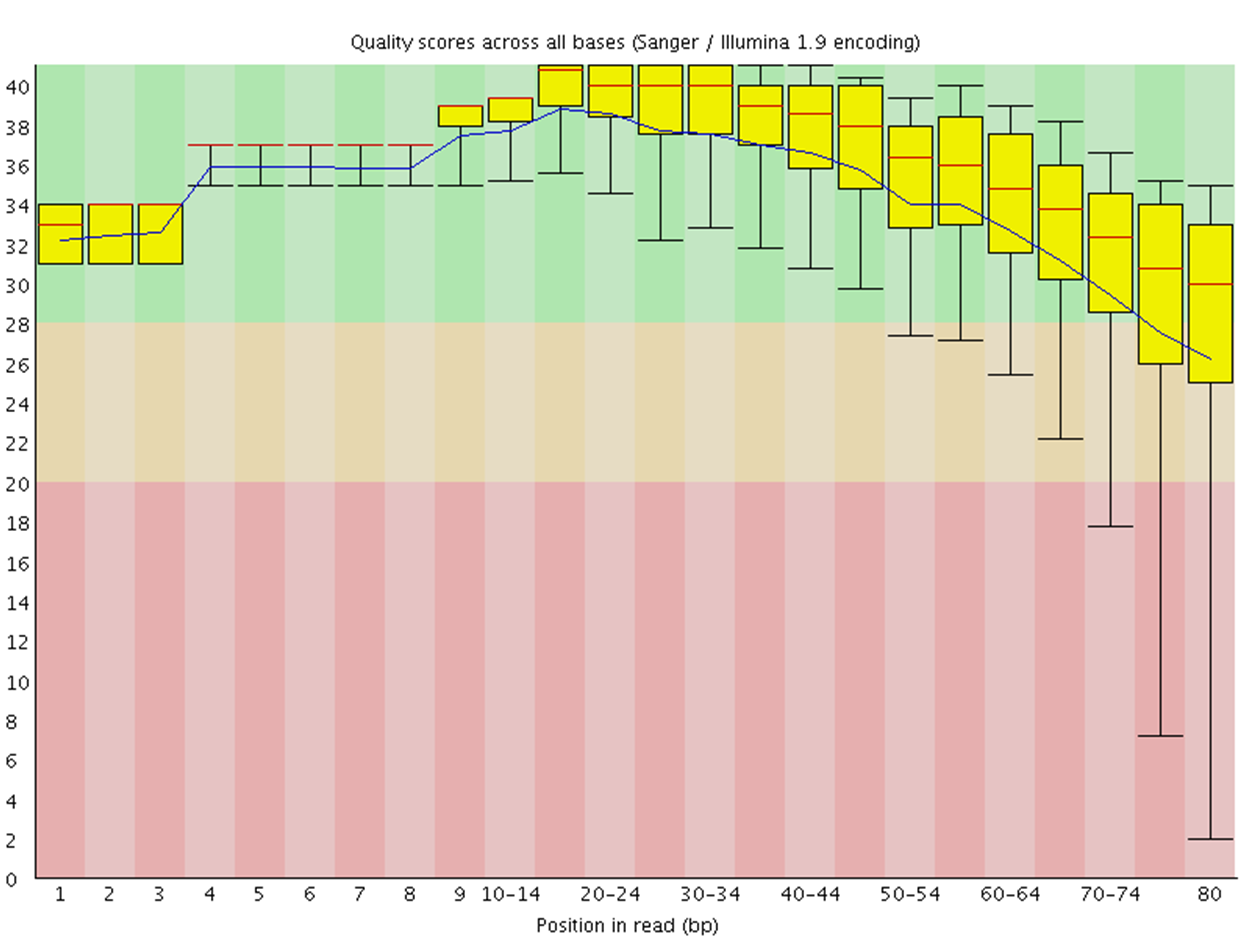
\includegraphics[width=0.8\textwidth]{ngs-qc/bad_example_trimmed_to_80bp.png}
\caption{Per base sequence quality plot for the fixed-length trimmed \texttt{bad\_example.fastq} reads.}
\label{fig:bad_example_trimmed_plot}
\end{figure}

\end{steps}

\begin{questions}
What values would you use for \texttt{-f} if you wanted to trim off 10 bases at
the 5' end of the reads?
\begin{answer}
\texttt{-f 11}
\end{answer}
\end{questions}

\subsection{Quality Based Trimming}
Base call quality scores can also be used to dynamically determine the trim
points for each read. A quality score threshold and minimum read length
following trimming can be used to remove low quality data.

\begin{steps}
Run the following command to quality trim your data:
\begin{lstlisting}
cd ~/QC
fastq_quality_trimmer -h
fastq_quality_trimmer -Q 33 -t 20 -l 50 -i bad_example.fastq -o bad_example_quality_trimmed.fastq
\end{lstlisting}
\end{steps}

\begin{steps}
Run FastQC on the quality trimmed file and visualise the quality scores.

\begin{lstlisting}
fastqc -f fastq bad_example_quality_trimmed.fastq
firefox bad_example_quality_trimmed_fastqc/fastqc_report.html &
\end{lstlisting}

The output should look like:

\begin{table}[H]
  \centering
  \caption{FastQC Basic Statistics table}
    \begin{tabular}{ll}
    \toprule
    Filename & bad\_example\_quality\_trimmed.fastq\\
    \midrule
    File type & Conventional base calls\\
    Encoding & Sanger / Illumina 1.9\\
    Total Sequences & 38976\\
    Filtered Sequences & 0\\
    Sequence length & 50-100\\
    \%GC & 48\\
    \bottomrule
    \end{tabular}
  \label{tab:badexamplequalitytrimmed}
\end{table}

\begin{figure}[H]
\centering
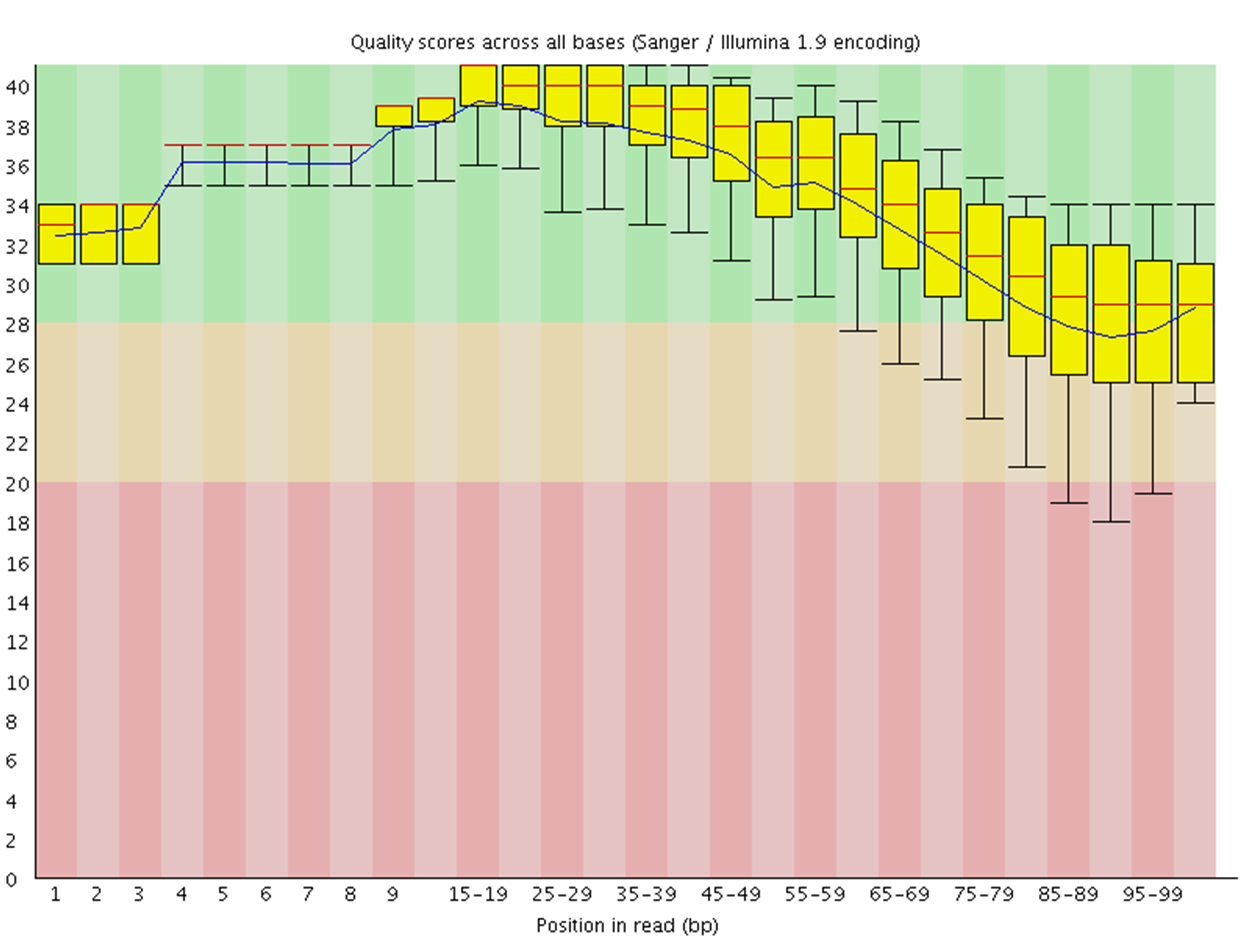
\includegraphics[width=0.8\textwidth]{ngs-qc/bad_example_quality_trimmed.png}
\caption{Per base sequence quality plot for the quality-trimmed \texttt{bad\_example.fastq} reads.}
\label{fig:bad_example_quality_trimmed_plot}
\end{figure}

\end{steps}

\begin{questions}
How did the quality score range change with two types of trimming?
\begin{answer}
Some poor quality bases (Q $<$20) are still present at the 3' end of the
fixed-length trimmed reads. It also removes bases that are good quality.

Quality-based trimming retains the 3' ends of reads which have good quality
scores.
\end{answer}

Did the number of total reads change after two types of trimming?
\begin{answer}
Quality trimming discarded $>$1000 reads. However, We retain a lot of maximal
length reads which have good quality all the way to the ends.
\end{answer}

What reads lengths were obtained after quality based trimming?
\begin{answer}
50-100

Reads $<$50 bp, following quality trimming, were discarded.
\end{answer}

Did you observe adapter sequences in the data?
\begin{answer}
No. (Hint: look at the overrepresented sequences.
\end{answer}

\end{questions}

\begin{advanced}
\subsection{Adapter Clipping}
Sometimes sequence reads may end up getting the leftover of adapters and primers
used in the sequencing process. It's good practice to screen your data for
these possible contamination for more sensitive alignment and assembly based
analysis.

\begin{note}
This is particularly important when read lengths can be longer than the
molecules being sequenced. For example when sequencing miRNAs.
\end{note}

Various QC tools are available to screen and/or clip these adapter/primer
sequences from your data. (e.g. FastQC, FASTX-Toolkit, cutadapt).

\begin{steps}
Here we are demonstrating \texttt{fastx\_clipper} to trim a given adapter
sequence.

\begin{lstlisting}
cd ~/QC
fastx_clipper -h
fastx_clipper -v -Q 33 -l 20 -M 15 -a GATCGGAAGAGCGGTTCAGCAGGAATGCCGAG -i bad_example.fastq -o bad_example_clipped.fastq
\end{lstlisting}
\end{steps}

\begin{note}
An alternative tool, not installed on this system, for adapter clipping is
\texttt{fastq-mcf}. A list of adapters is provided in a text file. For more
information, see FastqMcf at \url{http://code.google.com/p/ea-utils/wiki/FastqMcf}.
\end{note}

\subsection{Removing Duplicates}
Duplicate reads are the ones having the same start and end coordinates. This
may be the result of technical duplication (too many PCR cycles), or
over-sequencing (very high fold coverage). It is very important to put the
duplication level in context of your experiment. For example, duplication level
in targeted or re-sequencing projects may mean something different in RNA-seq
experiments. In RNA-seq experiments oversequencing is usually necessary when
detecting low abundance transcripts.

\begin{information}
The duplication level computed by FastQC is based on sequence identity at the
end of reads. Another tool, Picard, determines duplicates based on identical
start and end positions in SAM/BAM alignment files.

\textbf{We will not cover Picard but
provide the following for your information.}

Picard is a suite of tools for performing many common tasks with SAM/BAM format
files. For more information see the Picard website and information about the
various command-line tools available:

\url{http://picard.sourceforge.net/command-line-overview.shtml}
\end{information}

\begin{information}
Picard 1.69 is installed on this system in \texttt{/usr/share/java/picard-1.69/}

One of the Picard tools (MarkDuplicates) can be used to analyse and remove
duplicates from the raw sequence data. The input for Picard is a sorted
alignment file in BAM format. Short read aligners such as, bowtie, BWA and tophat
can be used to align FASTQ files against a reference genome to generate
SAM/BAM alignment format.
\end{information}

\begin{steps}
Interested users can use the following general command to run the
MarkDuplicates tool at their leisure. You only need to provide a BAM file for the
INPUT argument (not provided):


\begin{lstlisting}
cd ~/QC
java -jar /usr/share/java/picard/MarkDuplicates.jar INPUT=<alignment_file.bam> VALIDATION_STRINGENCY=LENIENT OUTPUT=alignment_file.dup METRICS_FILE=alignment_file.matric ASSUME_SORTED=true REMOVE_DUPLICATES=true

\end{lstlisting}
\end{steps}

\end{advanced}
